\documentclass[../main.tex]{subfiles}
\graphicspath{{\subfix{../img/}},{img},{img/ink}}
\begin{document}

\newgeometry{left=1cm, right=1cm}

\begin{landscape}
    \thispagestyle{empty}
    \section{Verlaufsplan}
    
    \begin{tabularx}{\linewidth}{ c@{\hspace{0.5cm}}p{4cm}@{\hspace{0.5cm}}X@{\hspace{0.5cm}}p{3cm}@{\hspace{0.5cm}}p{4cm}@{\hspace{0.5cm}} }
        \rowcolor{tablegray1} 
        \textbf{Uhrzeit} & \textbf{Phase} & \textbf{Unterrichtsschritte/Lehrer-Schülerinteraktion} & \textbf{Sozialform \& Arbeitsform} & \textbf{Matrialien} \\  
        \\[-5ex]
        \rowcolor{tablegray2} 
        10 min & Einstieg & Austeilen der iPads \newline Erklärung des Ablaufs \newline und Zeitplan \newline Erklärung einzelner Experimente &  Plenum & Beamer \\
        \\[-5ex]
        \rowcolor{tablegray1}
        45 min & Erarbeitung & SuS bearbeiten gewählte Station  & Gruppenarbeit & iPads \newline Stationen\\
        \\[-5ex]
        \rowcolor{tablegray2}
        20 min & Ergebnissicherung 1 & SuS präsentieren Ergebnisse \newline Zusammenstellen von Beobachtungen & Plenum & Beamer \\
    \\[-5ex]
        \rowcolor{tablegray1}
        15 min & Ergebnissicherung 2 & Tafelanschrieb \newline Hausaufgabe erklären & Plenum & Tafel
    \end{tabularx}

\begin{figure}[htpb]
    \centering
    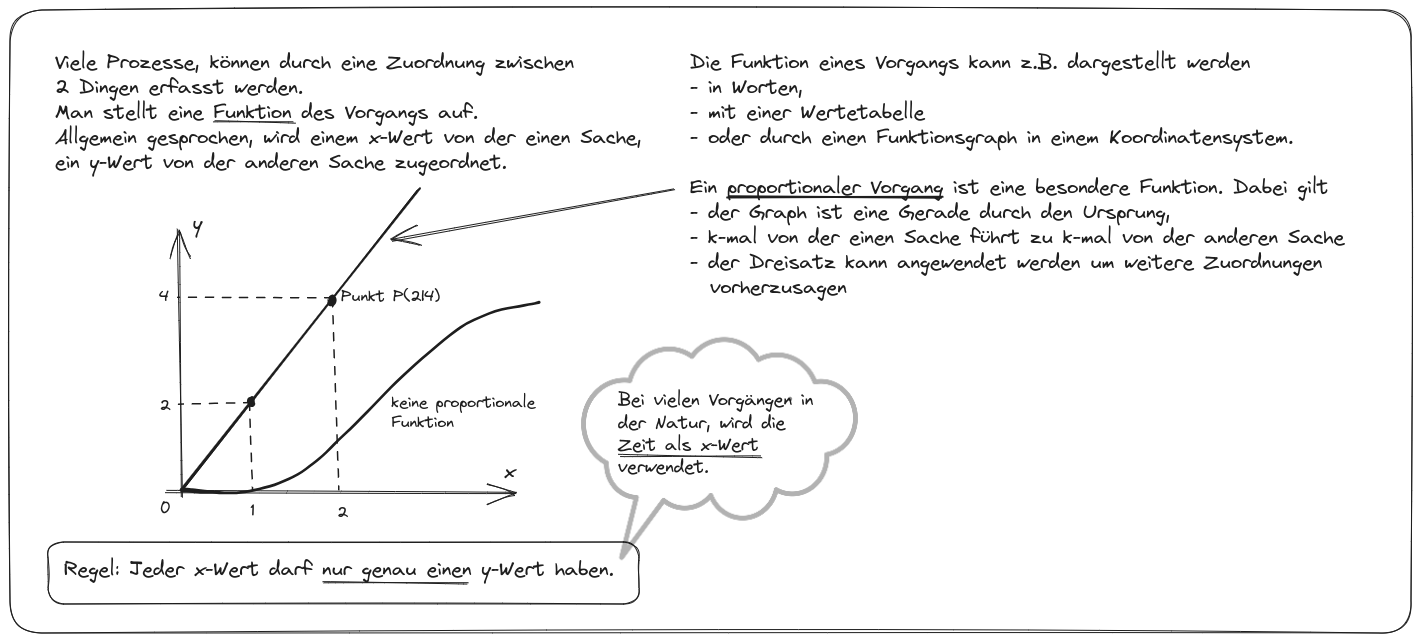
\includegraphics[width=0.8\textwidth]{img/tafelbild4.png}
\end{figure}
\end{landscape}

\restoregeometry
\end{document}
